\section{Using the Zephyr Environment}

\subsection{Build Sample}

Run the following inside the environment to compile the blinky sample.

\begin{itemize}
  \item For \textbf{WSL}:
  \begin{monobox}
cd ~/zephyrproject/zephyr/samples/basic/blinky/
west build --pristine --board @\board{}@ --build-dir /tmp/build
\end{monobox}
  \item For \textbf{Podman/Docker}:
  \begin{monobox}
cd ~/zephyrproject/zephyr/samples/basic/blinky/
west build --pristine --board @\board{}@ --build-dir ~/dev/build
\end{monobox}
\end{itemize}

\begin{infobox}
  When using WSL, we recommend to include the \mono{--build-dir /tmp/build} argument.
  If omitted the build system will compile the application in a \mono{build} folder in the current directory, which will be very slow when this directory is on the Windows file system (e.g. in \mono{/mnt/c/}).
\end{infobox}

\begin{infobox}
  When using Podman/Docker, setting the build directory to \mono{\~/dev/build} is necessary, otherwise you cannot access the binary from outside the container.
\end{infobox}

% container runtime: make sure builddir accessible

\newpage

\subsection{Flash Sample}

There are two main ways to flash an application to the target.
When first setting up the environment and testing with the blinky sample, you must always use the way described in \autoref{sec:jflash}.
The other way is only applicable if the project provides a \mono{.jlink} file.

\subsubsection{J-Flash Lite}\label{sec:jflash}
Start \emph{J-Flash Lite}, select the target device (\texttt{\mcu}), and make sure the \emph{Internal flash} flash bank is selected.

\begin{center}
  \begin{tikzpicture}
    \node [anchor=south west] {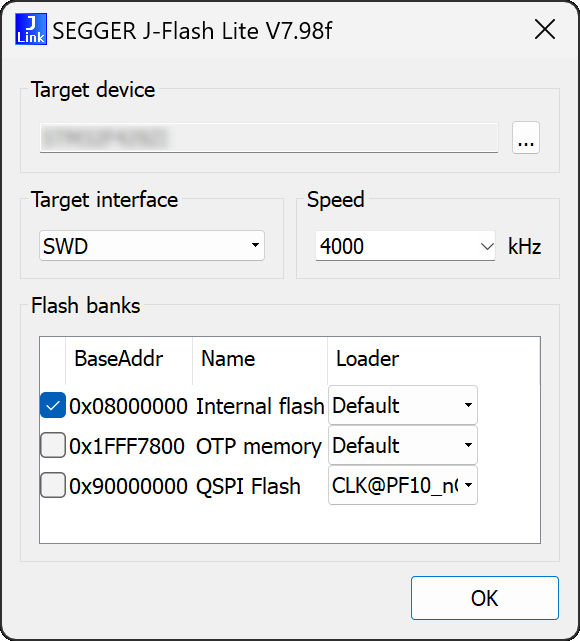
\includegraphics[width=8cm]{jflashlite.png}};
    \draw (7.39,7.1) [red,ultra thick] circle[radius=.4];
    \draw (.84,3.4) [red,ultra thick] circle[radius=.4];
  \end{tikzpicture}
\end{center}

In the next window select the firmware file (\mono{build/zephyr/zephyr.hex}) and click on \emph{Program Device}.

\begin{infobox}
  The WSL file system can be accessed in the explorer.
  \begin{center}
    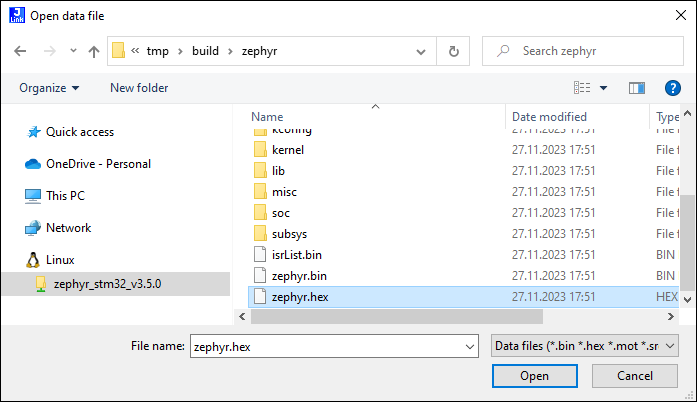
\includegraphics[width=.5\paperwidth]{explorer_wsl_hex}
  \end{center}

  It is possible, that the \emph{Linux} file system does not show up.
  If this is the case, it can be accessed by manually entering its path in the explorer:
  \mono{\\\\wsl\$}
  \begin{center}
    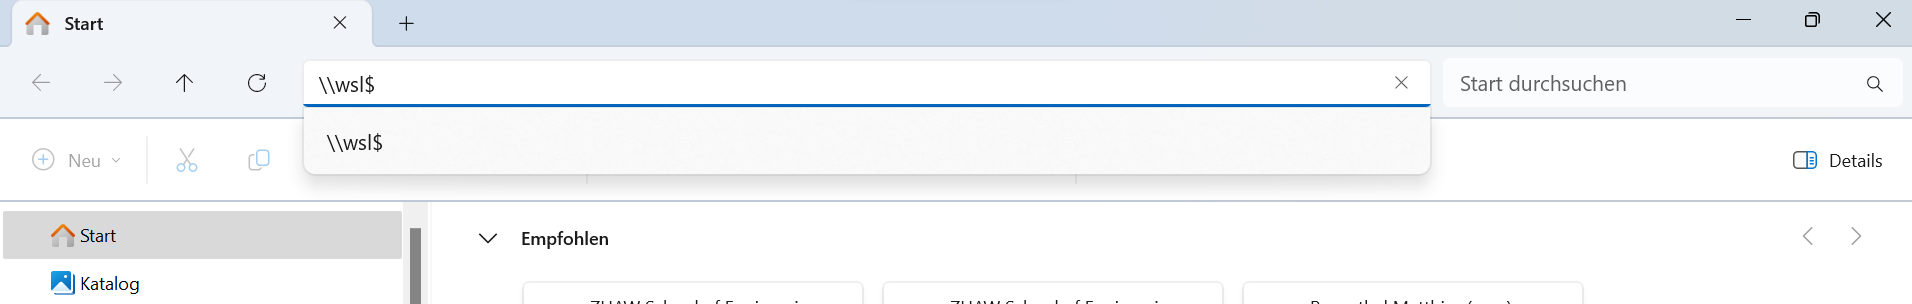
\includegraphics[width=.65\paperwidth]{win_file_explorer_wsl.png}
  \end{center}
  Press \emph{enter} to access the WSL file system.
\end{infobox}

\newpage

\subsubsection{J-Link Command File}
If a J-Link command file (\mono{.jlink}) is present in the project, it can be used to flash the binary from the command line.
On UNIX based systems the command to flash a binary with a J-Link command file is:

\begin{monobox}
JLinkExe -CommandFile path/to/file.jlink
\end{monobox}

On Windows the path to the J-Link executable needs to be added to the path environment variable first:

\begin{monobox}
$env:Path += ";C:\Program Files\SEGGER\JLink_<version>"
JLink -CommandFile path\to\file.jlink
\end{monobox}

\begin{infobox}
  Use the file explorer to get the right path to the JLink executable.
\end{infobox}

\begin{infobox}
  The above command to add the path is only for the current session.
  You can also add it permanently if you want.
\end{infobox}

\subsection{Test Flashed Sample}

Open a serial terminal with e.g. PuTTY to see the log output:

\begin{monobox}
plink -sercfg 115200 -serial com3
\end{monobox}

You might have to press the reset button on your microcontroller board to start the program and print the message again.

\begin{infobox}
  Open the device manager to find the COM-port number.
  \begin{center}
    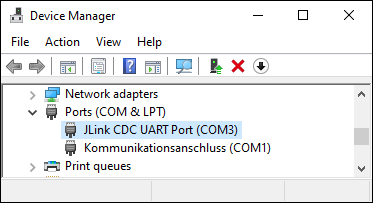
\includegraphics[width=.5\paperwidth]{device_manager_com}
  \end{center}
\end{infobox}
